% Seminário de 8 minutos — Aurora Solar. Compilar: latexmk -pdf slides.tex
\documentclass[aspectratio=169,10pt]{beamer}
\usetheme[progressbar=frametitle,numbering=fraction]{metropolis}
\usepackage[T1]{fontenc}
\usepackage[utf8]{inputenc}
\usepackage[brazil]{babel}
\usepackage{booktabs,tikz}
\usepackage[output-decimal-marker={,},per-mode=symbol]{siunitx}
\usetikzlibrary{arrows.meta,positioning}
\graphicspath{{figuras/}}
% Valores dos itens 19 e 29 gerados pelos scripts de fechamento; marcadores até a execução.
\IfFileExists{valores_i19.tex}{\newcommand{\CdValor}{\num{0.6215}}
\newcommand{\CdFaixa}{\num{0.6215} a \num{0.6338}}
\newcommand{\CdGCI}{\textnormal{GCI indeterminado}}
\newcommand{\CdA}{\SI{3.00}{m^2}}
\newcommand{\CdOscilatoria}{1}
\newcommand{\GCItabela}{\begin{table}[H]\centering\small
\caption{Item 19 --- coeficiente de arrasto na família final de três malhas.}
\begin{tabular}{llrrr}\toprule
Malha & Malha de fundo & Células & $h$ [m] & $C_d$ \\ \midrule
Fina & 55$\times$20$\times$10 & \num{750513} & \num{0.2447} & \num{0.621536} \\
Intermediária & 44$\times$16$\times$8 & \num{522986} & \num{0.2760} & \num{0.633751} \\
Grossa & 33$\times$12$\times$6 & \num{291219} & \num{0.3355} & \num{0.621971} \\
\bottomrule\end{tabular}\end{table}}
}{%
  \newcommand{\CdValor}{\textbf{[pendente]}}\newcommand{\CdFaixa}{\textbf{[pendente]}}\newcommand{\CdGCI}{\textbf{[pendente]}}%
  \newcommand{\CdA}{\textbf{[pendente]}}\newcommand{\GCItabela}{\textbf{[tabela GCI pendente]}}}
\IfFileExists{valores_i29.tex}{\newcommand{\PartidaMissao}{18h00}
\newcommand{\IbResposta}{Melhor combinação encontrada: velocidade \textbf{constante de \SI{20,5}{km/h}}, com partida às 18h00 (janela de 8\,h até 02h00); a viagem de \SI{7000}{km} termina em \textbf{214,8 dias} (\SI{32,6}{km/dia} em média) com reservas de 10\,\% na tração e 20\,\% nos serviços, ou 215,8 dias com reservas de 20/30\,\%.}
\newcommand{\IbResumo}{20,5 km/h constantes; 214,8 dias (31 km/dia em regime)}
\newcommand{\IbTexto}{%
A viagem parte com a tração cheia (\SI{98}{kWh} úteis) e o banco de serviços nominalmente cheio (\SI{14,4}{kWh} nominais) e só recebe energia solar. O tempo é contado a partir de 0h do primeiro dia, e a primeira partida é às 18h00: antes dela o veículo não roda, embora a janela diária de condução (18h00 a 02h00) cruze a meia-noite. A primeira chegada à reserva ocorre em 3,85 dias, após percorrer \SI{539}{km}; daí em diante cada dia roda o que o sol repôs, \SI{30,6}{km} em cerca de \SI{1,5}{h} de condução, bem abaixo do limite de 8\,h. Ao longo da viagem, os painéis geram \SI{3115}{kWh}: \SI{1300}{kWh} chegam à tração e \SI{1552}{kWh} abastecem a habitação (\SI{7,23}{kWh/dia}). A tração consome \SI{1383}{kWh} (\SI{0,198}{kWh/km}), em \SI{341}{h} de condução.

Como a energia solar diária é fixa, o tempo total é dominado pelos dias de espera para acumular energia, e não apenas pelas horas ao volante. O mínimo de consumo específico $v^{*}$ do item 27 é uma referência analítica para a busca; a agenda e as reservas ainda precisam ser verificadas. Nos casos comparados, rodar mais rápido aumenta o consumo e os dias de espera. Partir no fim da tarde deixa todo o período de sol com o veículo parado e os portáteis abertos. A Tabela~\ref{tab:i29comparacao} compara a melhor velocidade com 40 e \SI{80}{km/h} sob a mesma partida, as mesmas reservas e a mesma geração. A distância até a primeira vez que a tração atinge a reserva mede a autonomia com a bateria inicialmente cheia; o ritmo depois disso é o que a geração diária sustenta.
\IbComparacao

Em pista plana, o mínimo de consumo específico pode ser calculado diretamente (item 27), mas o tempo total também depende da agenda solar, da abertura dos portáteis, das reservas e da energia disponível em cada horário, interações que o simulador resolve intervalo a intervalo e que não têm forma fechada. Por isso a velocidade e o horário foram buscados numa grade; a velocidade publicada é a melhor combinação encontrada nas condições testadas, não um ótimo global demonstrado.

A melhor política foi localizada em duas etapas: varredura de \num{2784} combinações (\SIrange{12}{40}{km/h} a cada \SI{1}{km/h}, partida a cada \SI{0,5}{h}, duas reservas) com passo de \SI{5}{min}, e refino de \num{294} casos (passo de \SI{0,1}{km/h} e \SI{0,25}{h}) com passo de \SI{1}{min}; os líderes não estão na borda da grade local. Para o líder, entre passos de 5 e \SI{1}{min} a duração muda \SI{0,03}{dias}. A chegada é discretizada pela janela diária: se o último trecho não cabe antes do fim da janela, o veículo espera até a noite seguinte, de modo que uma pequena mudança de velocidade pode antecipar ou atrasar a chegada em quase um dia, como ocorre com as reservas de 20/30\,\%.

\textbf{Cenário opcional: acumular por mais de um dia.} Em vez de rodar todo dia o que o sol repôs, o veículo pode esperar alguns dias e percorrer um trecho maior depois, até 8\,h por dia. Essa política pode reduzir montagens, mas também altera o SOC, o espaço disponível nos bancos e o corte por capacidade; não se atribui a ela uma duração sem simulação específica. Devem ser mantidos o teto de 1560 Wp, o mínimo de 0,38 kW, as reservas e a ausência de energia da rede. A hipótese de dias claros repetidos, a recarga só pela interface CC e a operação diária dos portáteis continuam valendo; esse cenário não foi simulado.
\begin{figure}[H]\centering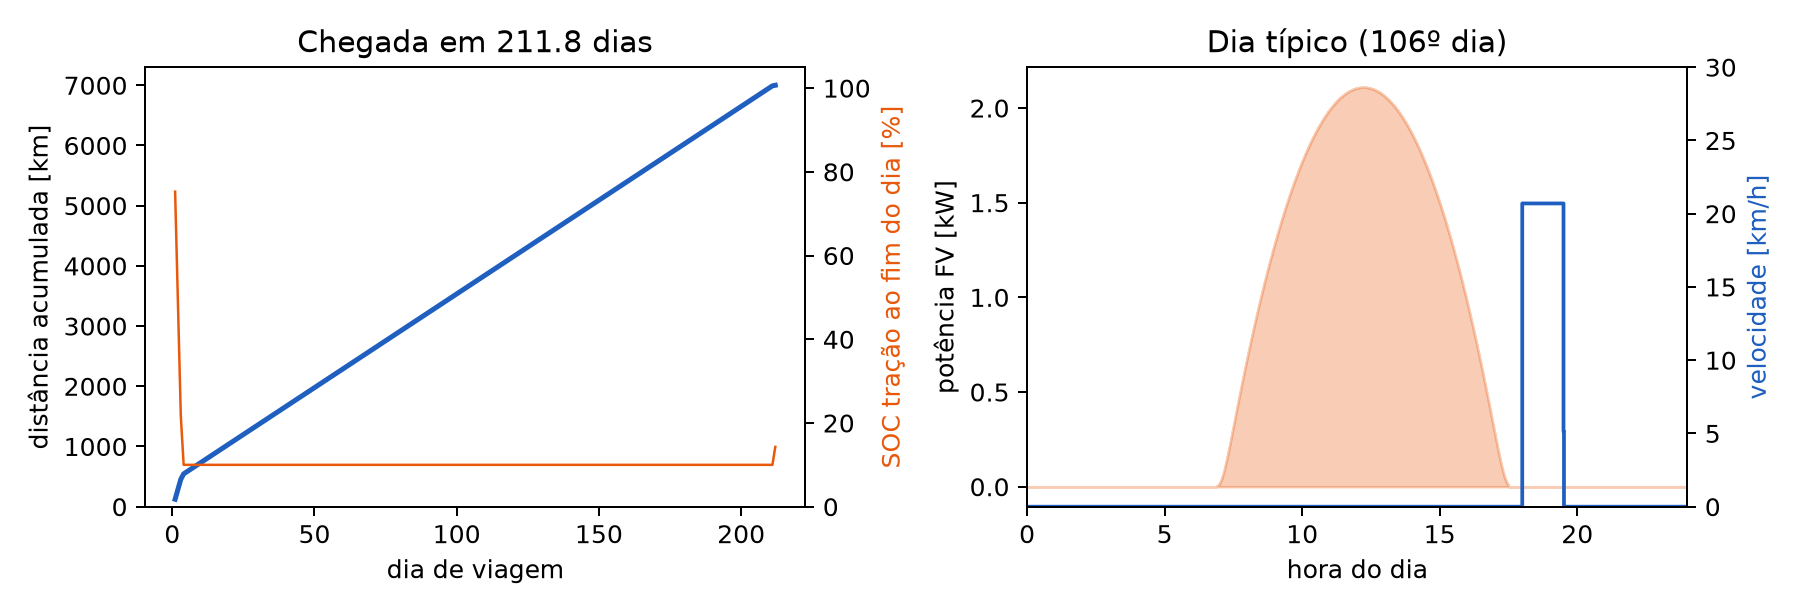
\includegraphics[width=\linewidth]{i29_missao.png}
\caption{Item 29 — distância acumulada e SOC da tração ao longo da viagem, e um dia típico.}\end{figure}}
\newcommand{\IbComparacao}{%
\begin{table}[H]\centering\small\setlength{\tabcolsep}{4pt}
\caption{Item 29 — mesma partida (18h00), mesmas reservas e mesma geração; só a velocidade muda.}
\label{tab:i29comparacao}
\begin{tabular}{rrrrrrr}
\toprule
$v$ & Viagem & Ao volante & Consumo & Até a reserva & \multicolumn{2}{c}{Depois da reserva} \\
{}[km/h] & [dias] & [h] & [kWh/km] & [km] & [km/dia] & [h/dia] \\
\midrule
20,5 & 214,8 & 341 & 0,198 & 539 & 30,6 & 1,49 \\
40,0 & 248,8 & 175 & 0,228 & 414 & 26,7 & 0,67 \\
80,0 & 457,8 & 88 & 0,408 & 216 & 14,8 & 0,19 \\
\bottomrule
\end{tabular}
\end{table}}
}{%
  \newcommand{\IbResposta}{\textbf{[pendente]}}\newcommand{\IbTexto}{}\newcommand{\IbResumo}{\textbf{[pendente]}}}

\definecolor{sol}{HTML}{E8590C}\definecolor{ceu}{HTML}{1F5FBF}
\setbeamercolor{frametitle}{bg=ceu}
\setbeamercolor{progress bar}{fg=sol}
\newcommand{\destaque}[1]{{\color{sol}\bfseries #1}}

\title{Aurora Solar}
\subtitle{Motorhome elétrico solar para duas pessoas — 35 itens}
\institute{Projeto de Modelagem e Simulação de Sistemas Térmicos e Fluídicos — EESC-USP}
\date{2 de dezembro de 2026}

\begin{document}
\maketitle

\begin{frame}{Conceito: furgão elétrico homologado + energia solar}
\begin{columns}[T]
\column{0.48\textwidth}
\begin{itemize}
\item Base \textbf{Fiat E-Ducato L3H2}, \SI{4250}{kg}: PMSM \SI{205}{kW}, LFP \SI{98}{kWh} úteis, limitador \SI{90}{km/h}
\item Teto: \destaque{4 Maxeon IBC, \SI{1540}{Wp}}
\item Portáteis: \destaque{4 $\times$ \SI{400}{W}} abertos com o veículo parado
\item Habitação em \SI{48}{V}: \SI{14,4}{kWh} LFP + inversor \SI{5}{kVA}
\item Sol $\to$ tração só por interface CC externa (CCS2) — \emph{hipótese}
\end{itemize}
\column{0.5\textwidth}
\centering
\begin{tikzpicture}[node distance=5mm and 7mm, every node/.style={draw, rounded corners, font=\scriptsize, align=center, minimum height=7mm}]
\node[fill=sol!20] (fv) {FV teto\\1540 Wp};
\node[fill=sol!20, below=of fv] (pt) {Portáteis\\1600 Wp};
\node[right=of fv] (mppt) {MPPT\\250/60 e 150/60};
\node[fill=ceu!15, right=of mppt] (srv) {Banco 48 V\\14,4 kWh};
\node[below=of srv] (inv) {Inversor\\220 V / 60 Hz};
\node[below=of inv] (casa) {Habitação\\7,2 kWh/dia};
\node[dashed, below=of mppt, yshift=-7mm] (cc) {Interface CC\\(hipótese, $\eta$ 0,9)};
\node[fill=ceu!15, below=of cc] (hv) {Bateria tração\\98 kWh, 400 V};
\draw[-{Stealth}] (fv) -- (mppt); \draw[-{Stealth}] (pt) -- (mppt);
\draw[-{Stealth}] (mppt) -- (srv); \draw[-{Stealth}] (srv) -- (inv); \draw[-{Stealth}] (inv) -- (casa);
\draw[-{Stealth}, dashed] (mppt) -- (cc); \draw[-{Stealth}, dashed] (cc) -- (hv);
\end{tikzpicture}
\end{columns}
\end{frame}

\begin{frame}{Projeto CAD: exterior, interior e configuração estacionada}
\begin{columns}[c]
\column{0.5\textwidth}
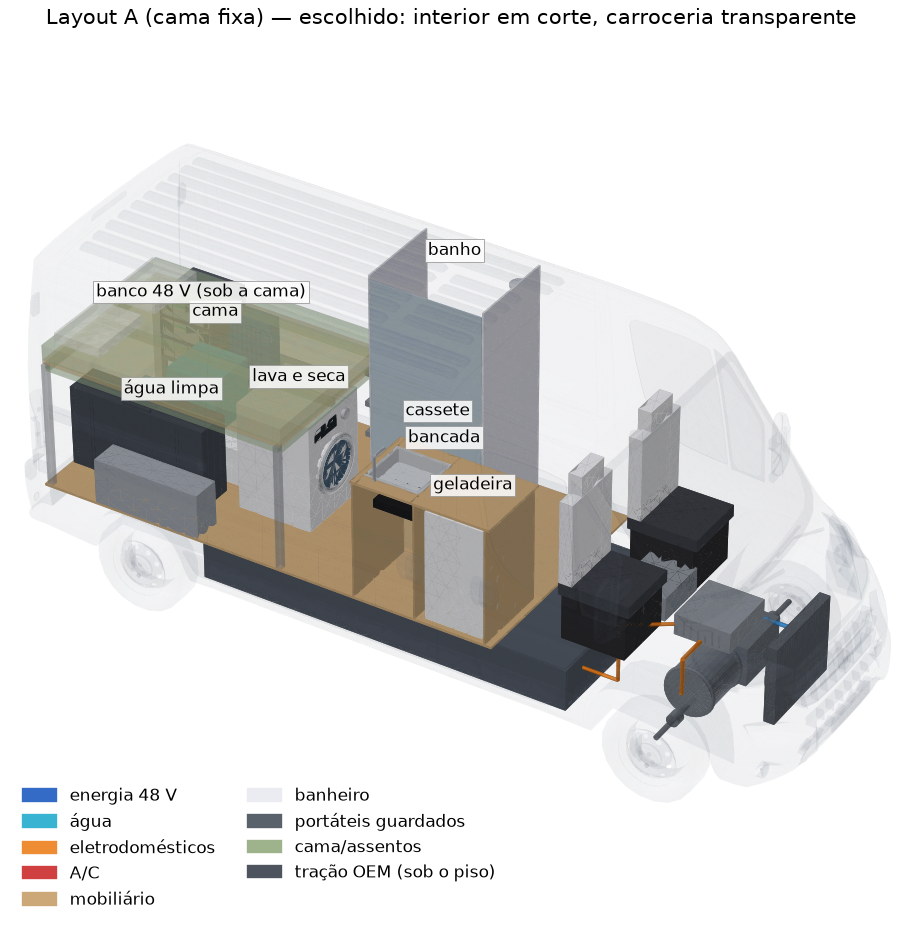
\includegraphics[width=\linewidth]{cad_interior_A.png}
\column{0.5\textwidth}
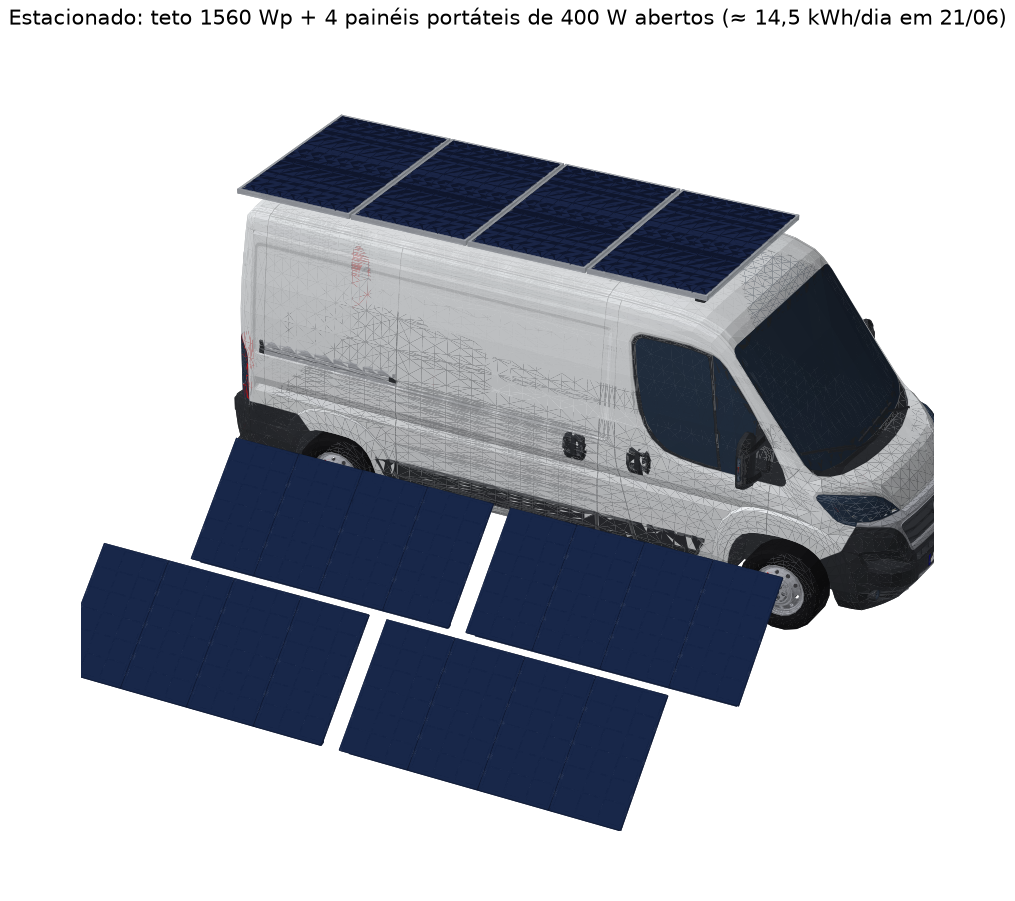
\includegraphics[width=\linewidth]{cad_estacionado.png}\\[2mm]
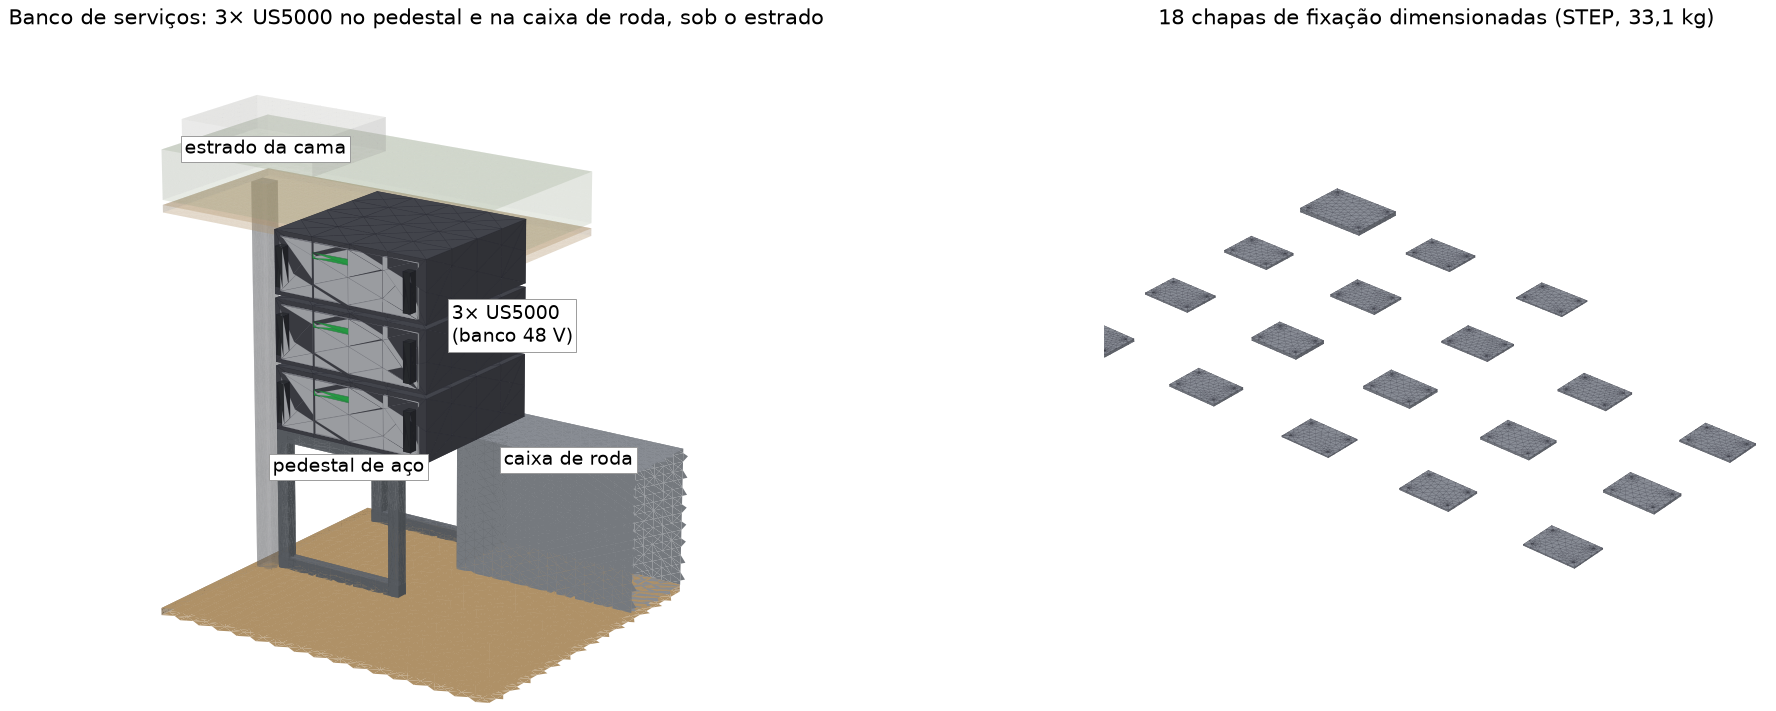
\includegraphics[width=0.8\linewidth]{cad_banco_fixacoes.png}
\end{columns}
\end{frame}

\begin{frame}{Especificações principais (itens 1--16)}
\small
\begin{columns}[T]
\column{0.5\textwidth}
\begin{tabular}{@{}ll@{}}
\toprule
Pneus & 225/75 R16C, 4,5/5,0 bar \\
Freios & discos ventilados \SI{300}{mm}, ABS \\
Motor & PMSM 205 kW / 410 N\,m \\
Transmissão & redutor fixo $i \approx 10$ \\
Baterias & 110/98 kWh + 14,4 kWh \\
Fiação & HV 120 mm²; 48 V até 120 mm² \\
Painéis & Maxeon 21,5--22,1\,\% \\
Controladoras & MPPT 99/98\,\%, inversor 96\,\% \\
\bottomrule
\end{tabular}
\column{0.5\textwidth}
\begin{tabular}{@{}ll@{}}
\toprule
Resfriamento & água-glicol, radiador \\
A/C & FreshWell 3000, 2,7 kW \\
Lubrificação & óleo do redutor, graxas \\
Interior & cama, banho, indução, 93 L \\
Suspensão & McPherson / feixe de molas \\
Chassi & 5,998 $\times$ 2,050 $\times$ 2,61 m \\
Carenagem & aço, isolamento 32 mm \\
Massa montada & \destaque{3976,5 kg} \\
\bottomrule
\end{tabular}
\end{columns}
\end{frame}

\begin{frame}{Aurora Solar}
\centering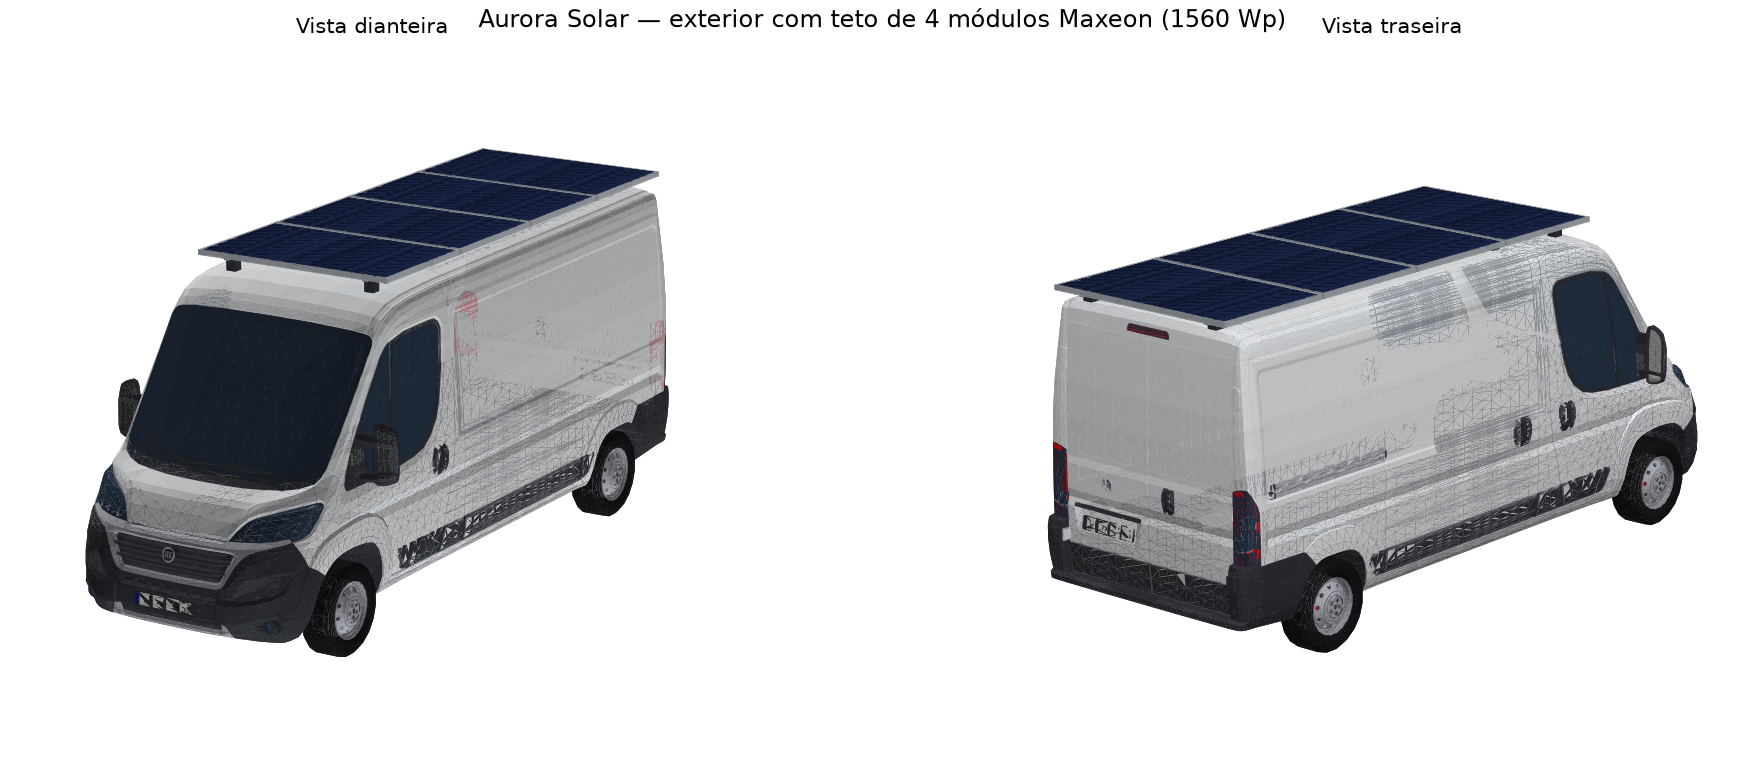
\includegraphics[width=\linewidth]{cad_exterior.png}
\end{frame}

\begin{frame}{Geometria (17) e aerodinâmica (19)}
\begin{columns}[c]
\column{0.58\textwidth}
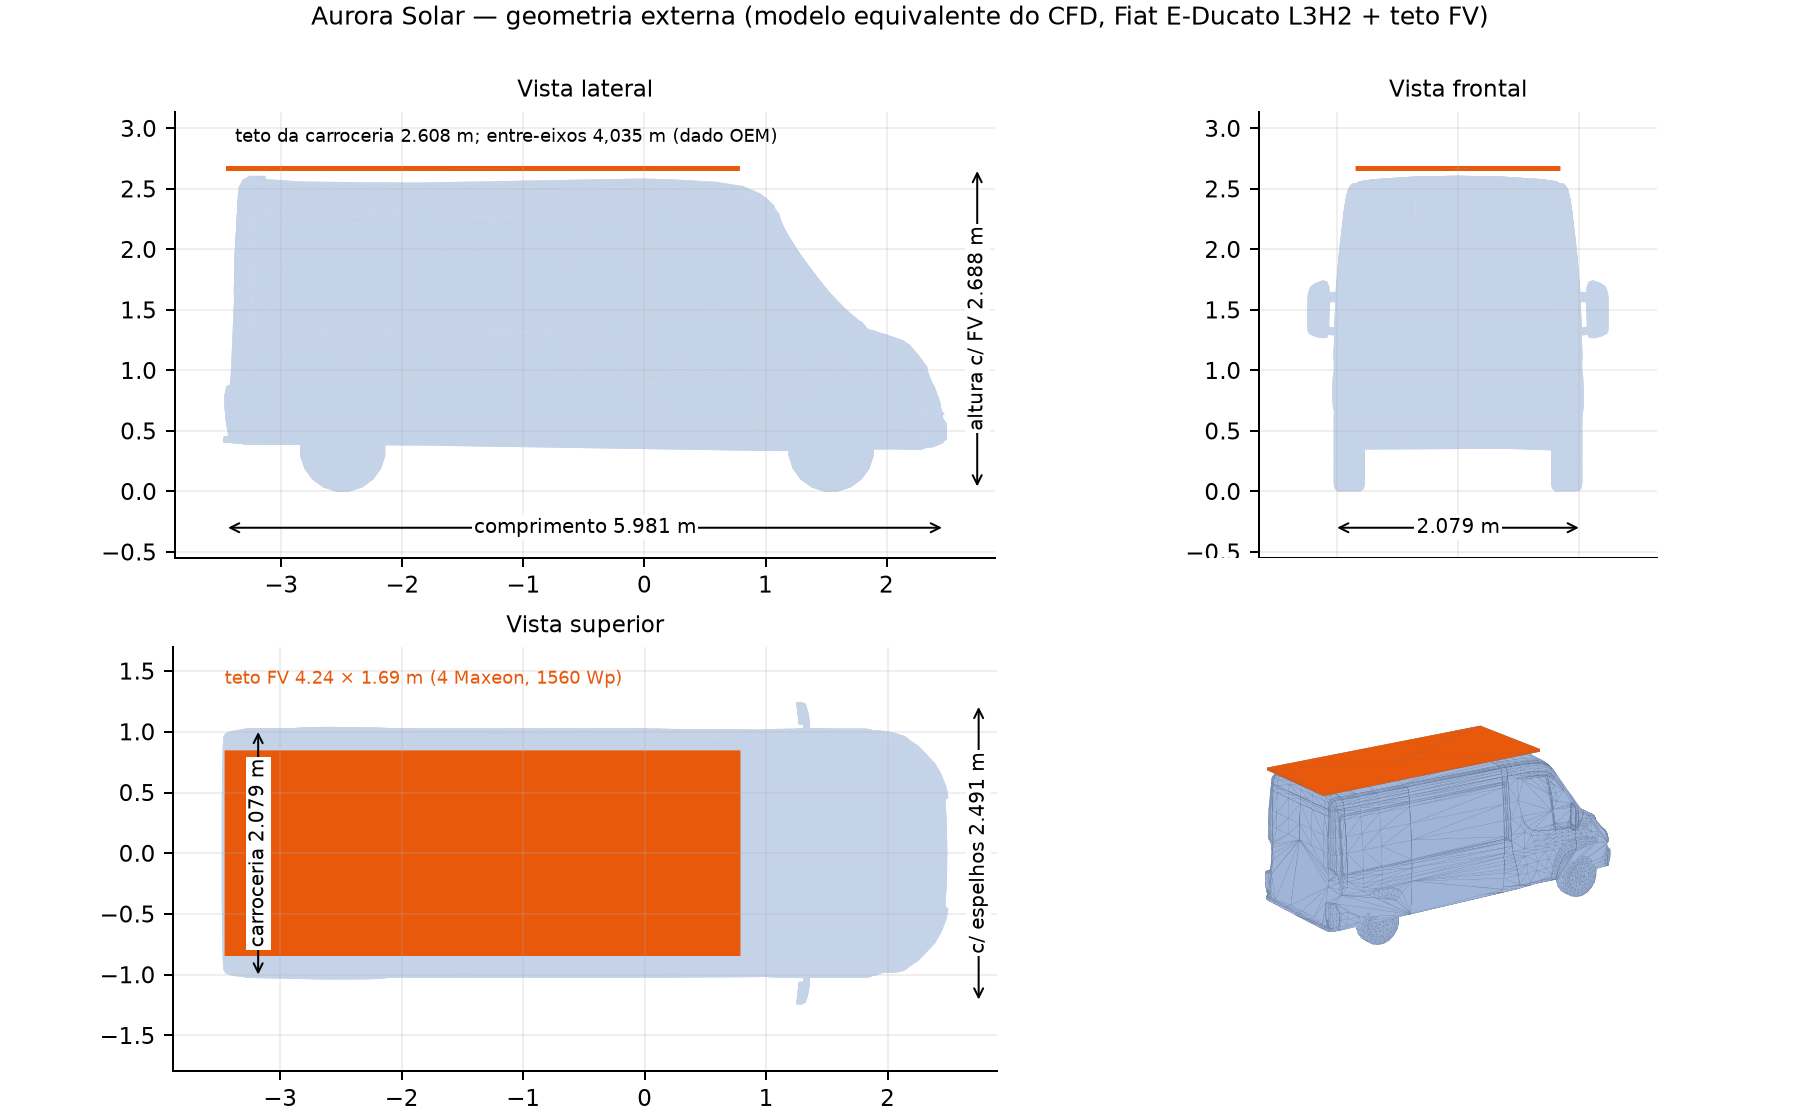
\includegraphics[width=\linewidth]{i17_vistas_exterior.png}
\column{0.4\textwidth}
\small
\begin{itemize}
\item CFD RANS $k$--$\omega$ SST, \SI{80}{km/h}, solo móvel
\item Família de 3 malhas sem limite de células
\item $A = \SI{4,828}{m^2}$
\item \destaque{$C_d = \CdValor$} (\CdGCI; convergência oscilatória)
\item $C_dA = \CdA$
\end{itemize}
\IfFileExists{figuras/i19_gci.png}{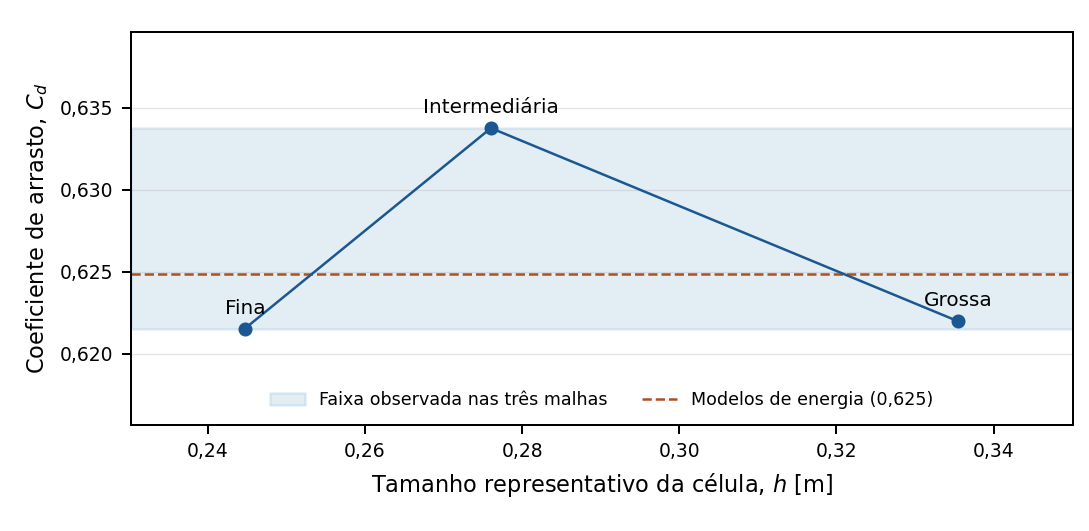
\includegraphics[width=\linewidth]{i19_gci.png}}{}
\end{columns}
\end{frame}

\begin{frame}{CFD: pressão na superfície e campo de velocidade (19)}
\includegraphics[width=0.9\linewidth]{cfd_cp.png}\\
\includegraphics[width=0.75\linewidth]{cfd_plano.png}
\end{frame}

\begin{frame}{Forças, potências e consumo (20--22, 26)}
\begin{columns}[c]
\column{0.5\textwidth}
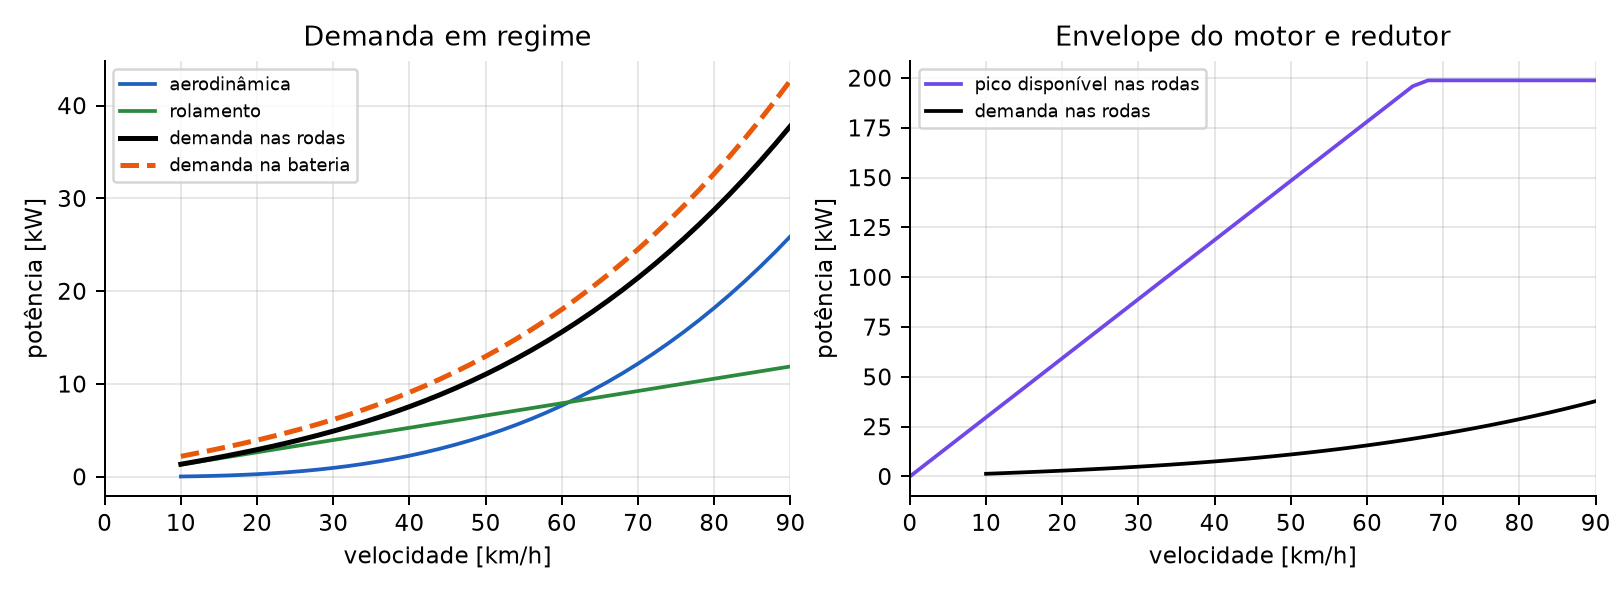
\includegraphics[width=\linewidth]{i22_potencias.png}
\column{0.48\textwidth}
\small
\begin{itemize}
\item $C_r = 0{,}012$; $F_r = \SI{468}{N}$
\item Arrasto supera rolamento acima de $\approx\SI{60}{km/h}$
\item Rodas: \SI{7,5}{kW} a 40 e \SI{28,6}{kW} a \SI{80}{km/h}
\item \destaque{\SI{4,44}{km/kWh} a 40 km/h}
\item \destaque{\SI{2,46}{km/kWh} a 80 km/h}
\end{itemize}
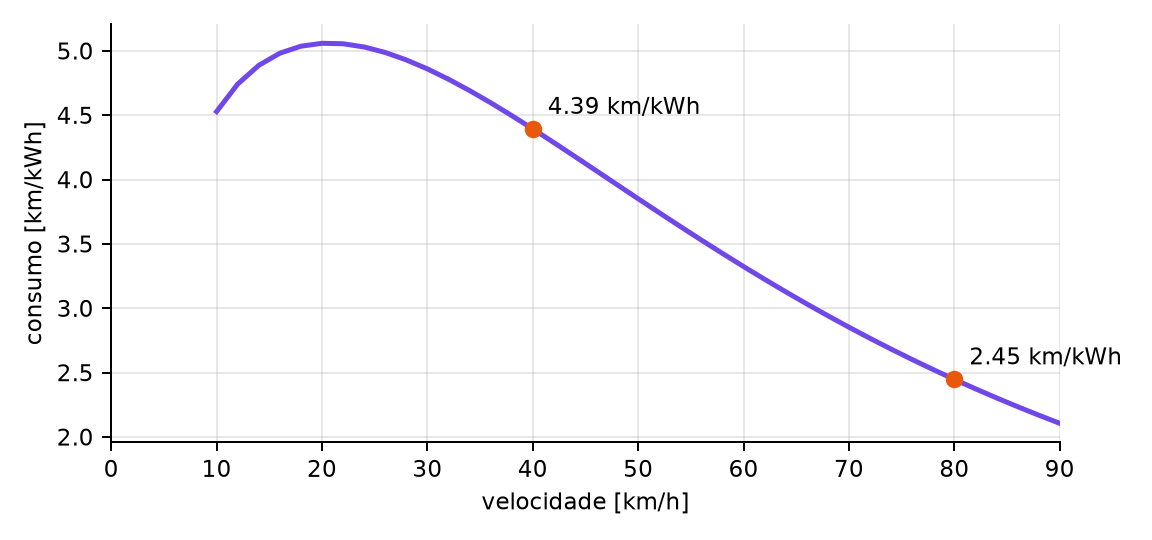
\includegraphics[width=0.85\linewidth]{i26_km_kwh.png}
\end{columns}
\end{frame}

\begin{frame}{Energia solar em 21/06 (8) e autonomia solar (25)}
\begin{columns}[c]
\column{0.5\textwidth}
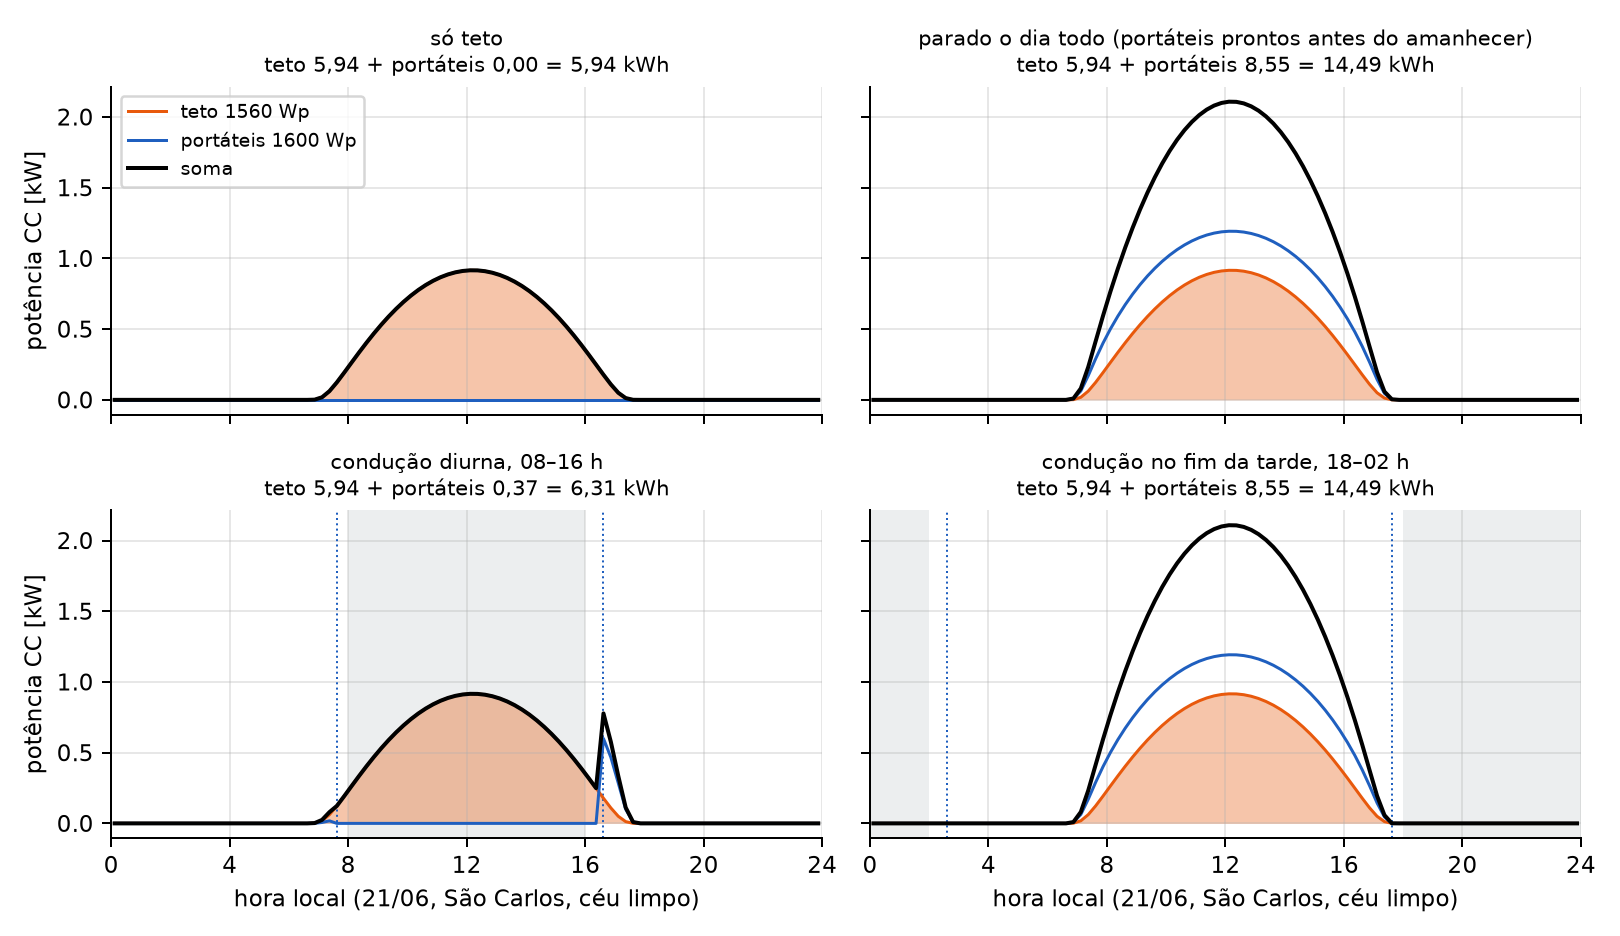
\includegraphics[width=\linewidth]{i08_geracao_solar.png}
\small Teto \SI{5,86}{kWh} + portáteis \SI{8,04}{kWh} = \destaque{\SI{13,9}{kWh/dia}}
\column{0.5\textwidth}
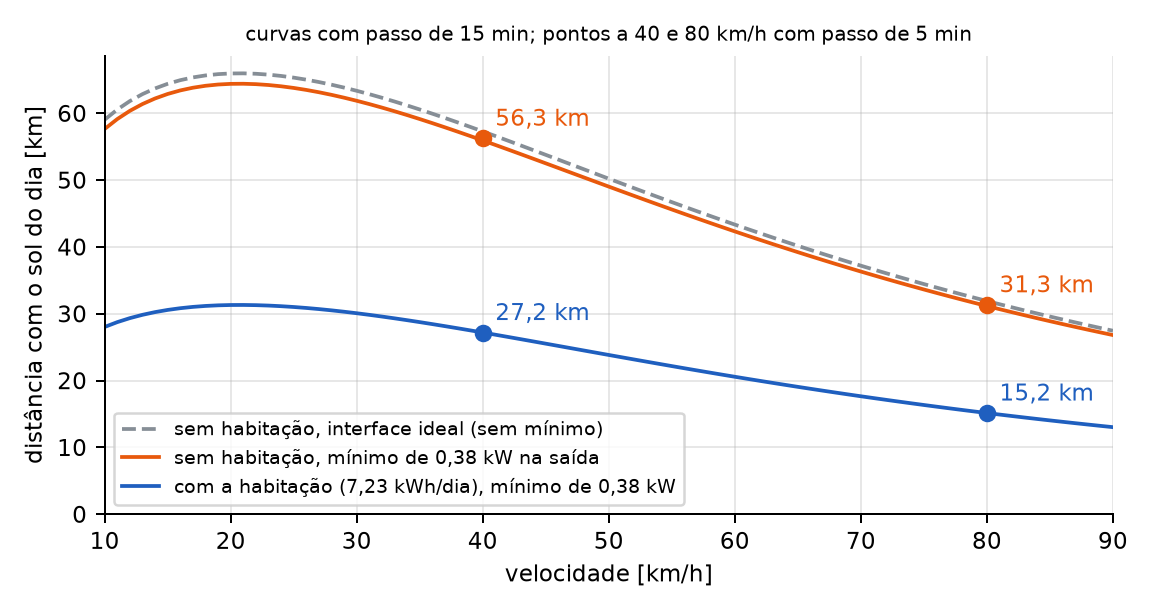
\includegraphics[width=\linewidth]{i25_autonomia_solar.png}
\small Só com o sol do dia: \destaque{\SI{57,6}{km} a 40} e \destaque{\SI{31,9}{km} a \SI{80}{km/h}}
\end{columns}
\end{frame}

\begin{frame}{Autonomia diária (27), velocidade máxima e 0--100 (28)}
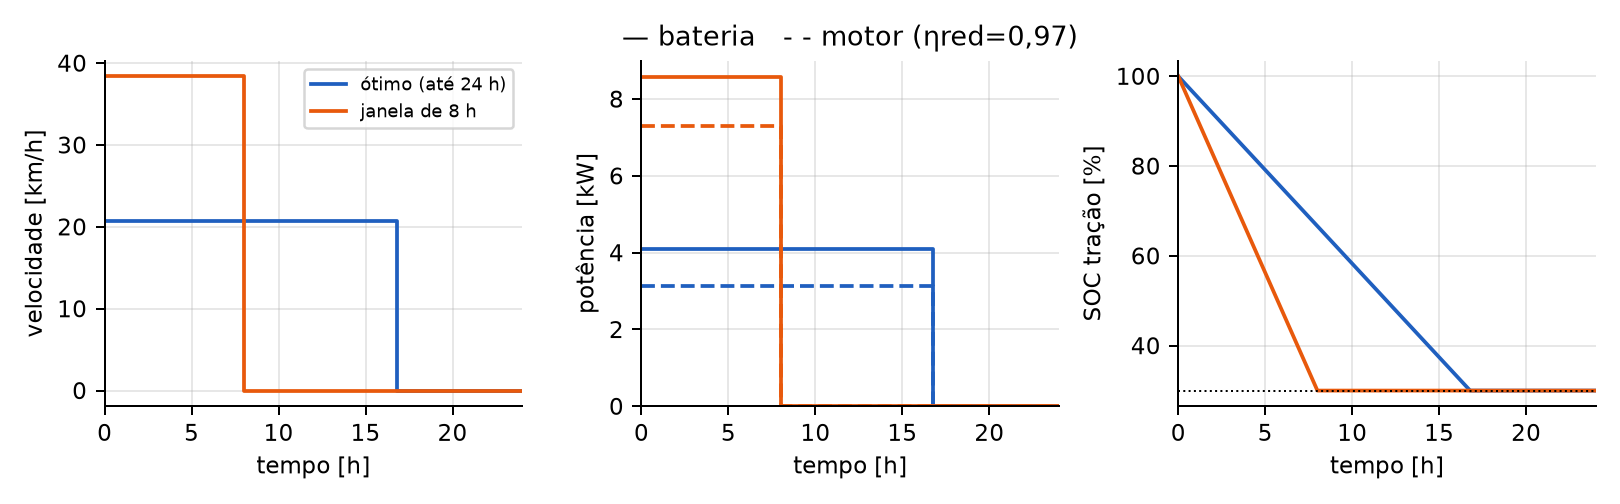
\includegraphics[width=\linewidth]{i27_perfil.png}
\small
\begin{columns}[T]
\column{0.5\textwidth}
SOC 100 $\to$ 30\,\%: \destaque{\SI{351,5}{km} a \SI{20,7}{km/h}} em 17\,h\\
(\SI{309,5}{km} em 8\,h a \SI{38,7}{km/h})\\
$v^{*} = (P_{aux}\eta/\rho C_d A)^{1/3}$ minimiza kWh/km
\column{0.5\textwidth}
$v_{max}$ = \SI{90}{km/h} (limitador de série)\\
0--100: \destaque{inalcançável}; 0--90 em \SI{10,6}{s}\\
(\SIrange{9,2}{14,2}{s} em 36 casos)
\end{columns}
\end{frame}

\begin{frame}{Belém--Chuí, \SI{7000}{km} só com bateria inicial e sol (29)}
\begin{columns}[c]
\column{0.62\textwidth}
\IfFileExists{figuras/i29_missao.png}{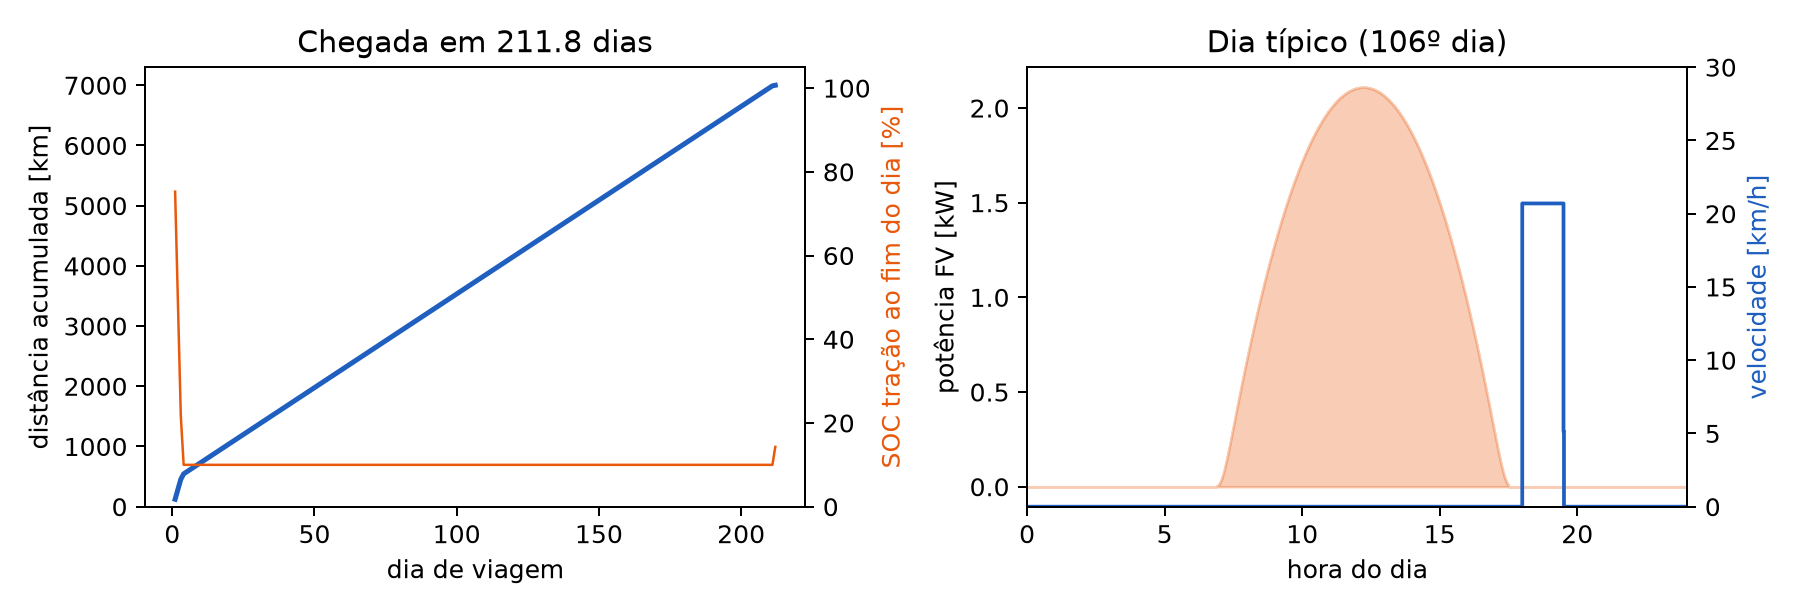
\includegraphics[width=\linewidth]{i29_missao.png}}{}
\column{0.36\textwidth}
\small
\begin{itemize}
\item Velocidade ótima \destaque{\SI{20,7}{km/h}} constante
\item Partida 17h45: o sol fica para os painéis
\item 4 dias gastando a bateria (\SI{567}{km})
\item Depois \SI{26}{km/dia} em $\approx\SI{1,3}{h}$
\item \destaque{\IbResumo}
\end{itemize}
\end{columns}
\end{frame}

\begin{frame}{Cabos do motor (30) e freios (33)}
\begin{columns}[c]
\column{0.5\textwidth}
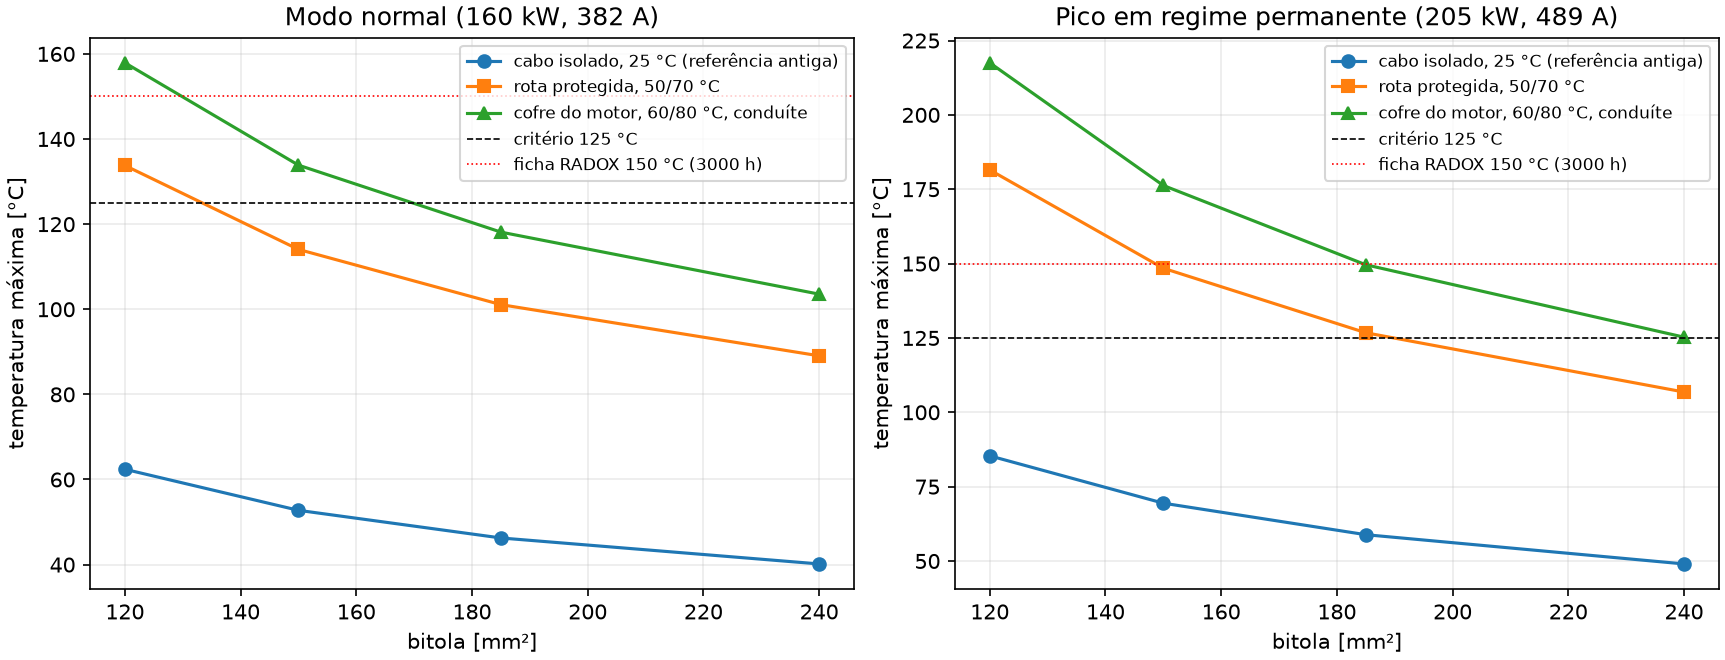
\includegraphics[width=\linewidth]{i30_cabos.png}
\small \SI{489}{A} RMS a \SI{205}{kW}: \destaque{\SI{158}{\celsius}\ (120 mm\textsuperscript{2}, cofre)}; \SI{118}{\celsius} com \SI{185}{mm^2}
\column{0.5\textwidth}
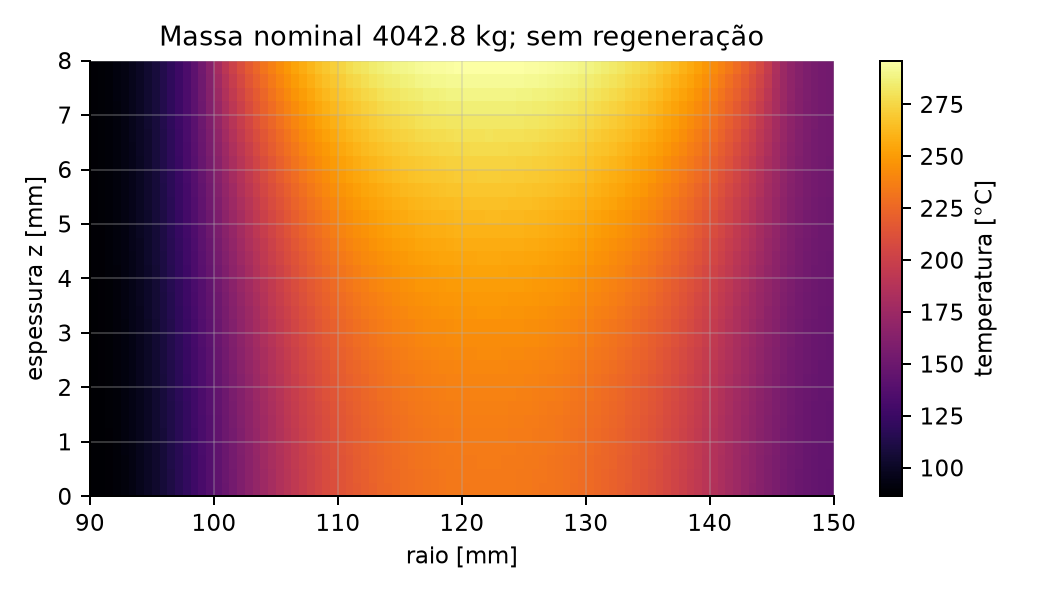
\includegraphics[width=\linewidth]{i33_campo.png}
\small 30 $\to$ 10 m/s em 5 s: \destaque{pico de \SI{293}{\celsius}}; \SI{213}{\celsius} com regeneração de 80 kW
\end{columns}
\end{frame}

\begin{frame}{Cabine fechada (31) e ar-condicionado (32)}
\begin{columns}[c]
\column{0.58\textwidth}
\includegraphics[width=\linewidth]{i31_cabine.png}
\column{0.4\textwidth}
\small
\begin{itemize}
\item Meio-dia, fechado, sem A/C: \destaque{\SI{49,1}{\celsius}} (zona única), \SI{50,3}{\celsius} médio no CFD 3D
\item 33 $\to$ \SI{25}{\celsius} com passageiros: \destaque{\SI{2,65}{kW}} de frio
\item \SI{2,87}{kW} com renovação de ar para CO$_2$
\item $\approx\SI{1,1}{kW}$ elétricos (COP 2,5)
\end{itemize}
\end{columns}
\end{frame}

\begin{frame}{Bateria em carga (34) e arrefecimento do motor (35)}
\begin{columns}[c]
\column{0.5\textwidth}
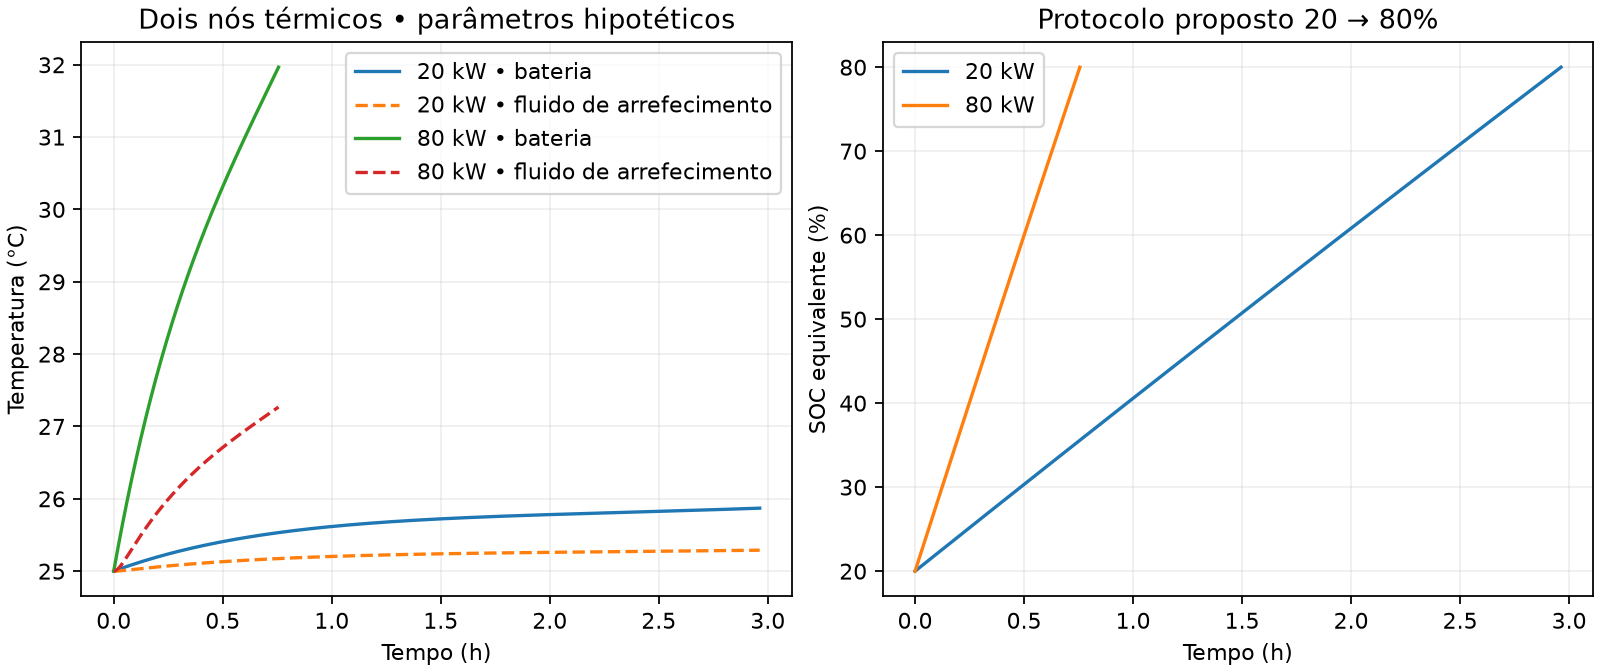
\includegraphics[width=\linewidth]{i34_bateria.png}
\small 20$\to$80\,\%: \destaque{\SI{25,9}{\celsius}} a 20 kW; \destaque{\SI{32,0}{\celsius}} a 80 kW
\column{0.5\textwidth}
\includegraphics[width=\linewidth]{i35_ponto_operacao.png}
\small Bomba: \destaque{\SI{31,9}{L/min}}, \SI{71,6}{kPa}, \SI{96}{W}; radiador rejeita \SI{22,9}{kW} (66,8 $\to$ \SI{55,1}{\celsius})
\end{columns}
\end{frame}

\begin{frame}{Custo com impostos de importação (24)}
\begin{columns}[c]
\column{0.55\textwidth}
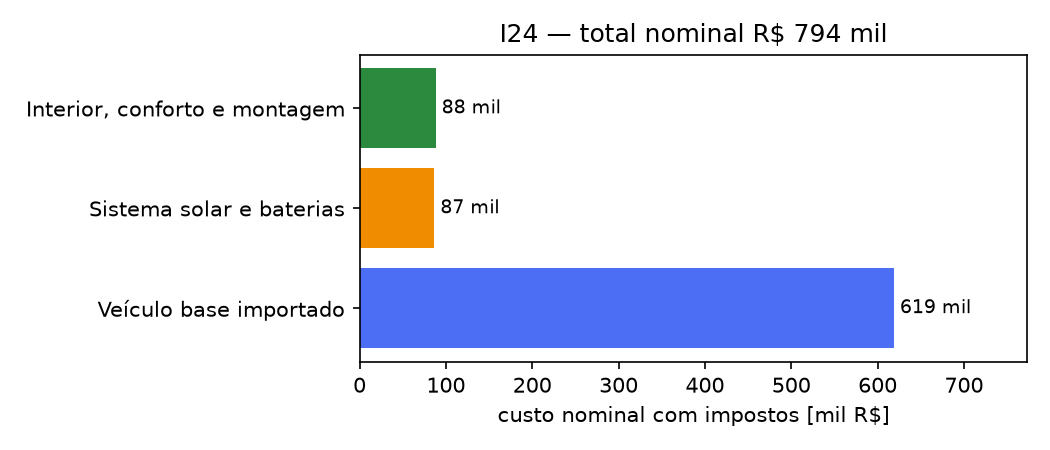
\includegraphics[width=\linewidth]{i24_custo.png}
\column{0.43\textwidth}
\small
\begin{itemize}
\item \destaque{R\$ 789 mil} (R\$ 721--882 mil)
\item Veículo importado: R\$ 619 mil (II 35\,\%)
\item Conversão: R\$ 170 mil
\item Tributos de importação: R\$ 324 mil
\end{itemize}
\end{columns}
\end{frame}

\begin{frame}{Conclusões}
\begin{itemize}
\item O sol de inverno (\SI{13,9}{kWh/dia}) sustenta a \destaque{habitação} (\SI{7,2}{kWh/dia}) com folga
\item Para a \destaque{tração} de um furgão de \SI{4}{t}, um dia de sol vale \SIrange{32}{58}{km}
\item Menor tempo = menor consumo por km: \SI{20,7}{km/h}, \IbResumo
\item Térmica dos cabos \destaque{depende do contorno}: 120 mm\textsuperscript{2} chega a \SI{158}{\celsius} no cofre; solução \SI{185}{mm^2} ou limitar a potência contínua
\item Limitações: interface CC solar--tração não autorizada pelo fabricante; mapas OEM não publicados; sem validação experimental
\end{itemize}
\vfill
\centering\small Código e resultados: \url{https://github.com/MHC-CodeSmith/STF_MotorHome}
\end{frame}

\end{document}
